\chapter{はじめに}
\label{ch:introduction}

%% ============================================================
%%  1.1 最適輸送とは何か
%% ============================================================
\section{最適輸送とは何か}
\label{sec:what-is-ot}

科学や日常生活における多くの意思決定は，\textbf{最短経路の原理}に導かれている．
ある地点にある品物を別の地点に届けたいとき，最も少ない労力で済む方法を選ぶのは自然な発想であり，
平面上であれば直線に沿って，より一般の距離空間であれば測地線に沿って移動させることがこれに当たる．

\textbf{最適輸送}（optimal transport; OT）の理論は，この直感を大きく一般化する．
すなわち，1つの品物だけを運ぶのではなく，\textbf{複数の品物}（あるいはその連続的な分布）を
ある配置からべつの配置へと同時に移動させる問題を扱う．
1人の個人を目的地に送ることは単純であるが，集団全体を別の配置へ移動させ，
しかも到着時に所定の分布が実現されるようにすることは，はるかに複雑な問題となる．
この問題を数学的に定式化するには，測度論・凸最適化・線形計画法などの道具が必要となる．

以下に，最適輸送の概念を直感的に把握するための2つの具体例を挙げる．

\begin{example}{砂山の移動 --- Monge の原問題}{sand-pile}
  地面のある場所に砂山（土砂の山）があり，これを掘り返して別の場所に所定の形状で盛り上げたいとする．
  砂の総量は保存されるものとする（掘り出した砂の総量 $=$ 盛り上げた砂の総量）．

  このとき，「どの砂粒をどこに運ぶか」という輸送計画を立て，
  輸送にかかる\textbf{総コスト}（$=$（各砂粒の質量）$\times$（移動距離）の総和）を
  最小化する問題が，1781年に Monge が提唱した最適輸送の原問題である．

  ここで重要な点は，各砂粒は\textbf{1つの行き先}にしか運べないという制約である．
  すなわち，砂粒を分割して複数の場所に送ることは許されない．
\end{example}

\begin{example}{工場と倉庫の輸送計画 --- Hitchcock--Kantorovich 問題}{factory-warehouse}
  $n$ 箇所の倉庫がそれぞれ供給量 $a_1, \ldots, a_n$ の商品を保有し，
  $m$ 箇所の工場がそれぞれ需要量 $b_1, \ldots, b_m$ の商品を必要としているとする．
  供給量の合計と需要量の合計は等しいと仮定する：$\sum_{i=1}^n a_i = \sum_{j=1}^m b_j$．

  倉庫 $i$ から工場 $j$ へ1単位の商品を輸送するコストが $C_{i,j} \geq 0$ で与えられているとき，
  輸送計画 $P_{i,j} \geq 0$（倉庫 $i$ から工場 $j$ へ送る量）を求めて，
  \textbf{総輸送コスト}
  \[
    \sum_{i=1}^n \sum_{j=1}^m C_{i,j} P_{i,j}
  \]
  を最小化したい．ただし，供給制約 $\sum_{j=1}^m P_{i,j} = a_i$ と
  需要制約 $\sum_{i=1}^n P_{i,j} = b_j$ を満たす必要がある．

  この定式化では，Monge の問題と異なり，1つの倉庫の商品を\textbf{複数の工場に分割して}
  送ることが許される．これは Kantorovich による緩和の考え方に対応しており，
  問題が線形計画問題となるため，効率的に解くことが可能となる．
\end{example}

以上の例が示すように，最適輸送は，「品物の分布」どうしを比較し，
一方の分布を他方の分布に変換するための最小コストを求めるという枠組みである．
この最小コストは，確率分布の空間に自然な\textbf{距離}（Wasserstein 距離）を定め，
機械学習・画像処理・統計学・経済学など多くの分野で強力なツールとなっている．

%% ============================================================
%%  1.2 歴史的背景
%% ============================================================
\section{歴史的背景}
\label{sec:history}

最適輸送の理論は約240年にわたる歴史を持つ．以下に主要な発展を概観する．

\subsection*{Monge (1781)}

最適輸送の起源は，フランスの数学者 Gaspard Monge が1781年に発表した
``M\'{e}moire sur la th\'{e}orie des d\'{e}blais et des remblais''
（土砂の切り盛りに関する覚書）に遡る．
Monge は，ある場所から掘り出した土砂を別の場所に運んで盛り上げるとき，
総輸送コストを最小にする方法を求める問題を定式化した．
この定式化では，各々の土砂の微小部分は\textbf{決定論的に}1つの行き先に送られる．
すなわち，輸送は写像 $T\colon \X \to \Y$ によって記述される（\ref{sec:monge-overview}~節で詳述）．

しかしながら，Monge の定式化には数学的な困難がある．
実行可能な写像の集合は一般に凸でなく，
また実行可能な写像が存在しない場合すらある（\ref{sec:monge-overview}~節の例 \ref{ex:monge-nonexistence} を参照）．
このため，Monge の問題は長い間未解決のまま残された．

\subsection*{Tolstoi (1930) と Hitchcock (1941)}

20世紀に入り，最適輸送は実用的な文脈で再発見された．
Tolstoi (1930) はソビエト連邦における輸送ネットワークの最適化を研究し，
Hitchcock (1941) は独立に工場・倉庫間の輸送問題を線形計画として定式化した．
これらの研究は，最適輸送が純粋数学のみならず，
物流・生産計画・ネットワーク設計といった応用上の重要な問題であることを示した．

\subsection*{Kantorovich (1942)}

ソビエトの数学者・経済学者 Leonid Kantorovich（1975年ノーベル経済学賞受賞）は，
1942年に最適輸送問題の革命的な再定式化を提案した．
Monge の定式化では輸送が決定論的な写像 $T$ で記述されるのに対し，
Kantorovich は輸送を\textbf{カップリング測度} $\pi$（結合確率測度）で記述する\textbf{緩和}を導入した
（\ref{sec:kantorovich-overview}~節で詳述）．

この緩和の核心的な意義は以下の点にある：
\begin{itemize}
  \item カップリング測度の集合は\textbf{凸集合}であり，目的関数はそれに関して線形である．
  \item したがって，Kantorovich の定式化は\textbf{線形計画問題}であり，常に解が存在する．
  \item さらに，線形計画の双対理論から\textbf{双対問題}が得られ，これは最適輸送の幾何学的理解に重要な役割を果たす．
\end{itemize}

\subsection*{Brenier (1991) と現代の発展}

1991年に Yann Brenier は，$\R^d$ 上の二次コスト $c(x,y) = \norm{x-y}_2^2$ に対して，
最適輸送写像が存在し，凸関数の勾配として一意的に表されることを証明した（Brenier の定理）．
この結果は，最適輸送を\textbf{凸解析}，\textbf{偏微分方程式}（Monge--Amp\`{e}re 方程式），
\textbf{流体力学}と深く結びつけ，最適輸送の理論を飛躍的に発展させた．

21世紀に入ると，計算手法の進展（特に Sinkhorn アルゴリズムによるエントロピー正則化）により，
最適輸送は大規模な実データにも適用可能となった．
現在では，画像処理（テクスチャ合成，色転写），機械学習（生成モデル，ドメイン適応），
自然言語処理，計算生物学，経済学など幅広い分野で活用されている．

%% ============================================================
%%  記法
%% ============================================================
\section*{記法}
\label{sec:notation}

\begin{itemize}
  \item $\range{n}$：整数の集合 $\{1, \ldots, n\}$．

  \item $\ones_{n,m}$：すべての成分が $1$ である $\R^{n \times m}$ 上の行列．
    $\ones_n$：すべての成分が $1$ の $n$ 次元ベクトル．

  \item $\Identity_n$：$n \times n$ 単位行列．

  \item $\diag(\mathbf{u})$：ベクトル $\mathbf{u} \in \R^n$ に対し，
    対角成分が $u_1, \ldots, u_n$ で非対角成分が $0$ の $n \times n$ 行列．

  \item $\simplex_n$：$n$ 次元確率単体．
    すなわち $\R_+^n$ における確率ベクトルの集合
    $\left\{ \mathbf{a} \in \R_+^n \mid \sum_i a_i = 1 \right\}$．

  \item $(\mathbf{a}, \mathbf{b})$：
    確率単体 $\simplex_n \times \simplex_m$ に属するヒストグラム．

  \item $(\alpha, \beta)$：空間 $(\X, \Y)$ 上の測度．

  \item $\frac{\d\alpha}{\d\beta}$：
    測度 $\alpha$ の $\beta$ に関する相対密度（ラドン--ニコディム導関数）．

  \item $\rho_\alpha = \frac{\d\alpha}{\d x}$：
    ルベーグ測度に関する測度 $\alpha$ の密度．

  \item $\left(\alpha = \sum_i a_i \delta_{x_i},\;
    \beta = \sum_j b_j \delta_{y_j}\right)$：
    台 $x_1, \ldots, x_n \in \X$ および $y_1, \ldots, y_m \in \Y$ 上の離散測度．

  \item $c(x, y)$：基底コスト関数．
    対応するペアワイズコスト行列 $C_{i,j} = c(x_i, y_j)$．

  \item $\pi$：$\alpha$ と $\beta$ のカップリング測度．
    離散測度に対しては $\pi = \sum_{i,j} P_{i,j} \delta_{(x_i, y_j)}$
    であり，輸送行列 $\mathbf{P}$ として記述される．

  \item $\Couplings(\alpha, \beta)$：カップリング測度の集合．
    離散版は $\CouplingsD(\mathbf{a}, \mathbf{b})$．

  \item $T \colon \X \to \Y$：Monge 写像．
    $T\pushforward \alpha = \beta$ を満たす．

  \item $(\mathbf{f}, \mathbf{g})$：
    双対変数（双対ポテンシャル）．

  \item $\MKD_{\mathbf{C}}(\mathbf{a}, \mathbf{b})$
    および $\MK_c(\alpha, \beta)$：
    コスト $\mathbf{C}$（ヒストグラム）および $c$（任意の測度）に対する
    最適輸送問題の最適値．

  \item $\WassD_p(\mathbf{a}, \mathbf{b})$
    および $\Wass_p(\alpha, \beta)$：
    距離行列 $\mathbf{D}$（ヒストグラム）および距離 $d$（任意の測度）に対する
    $p$-Wasserstein 距離．

  \item $\inner{\cdot}{\cdot}$：
    ベクトルに対してはユークリッド内積．
    同じサイズの行列 $A, B$ に対しては
    $\inner{A}{B} \defeq \tr(A^\top B)$（フロベニウス内積）．

  \item $f \oplus g(x, y) \defeq f(x) + g(y)$：
    関数 $f \colon \X \to \R$，$g \colon \Y \to \R$ に対する直和．
    離散版では $\mathbf{f} \oplus \mathbf{g}
    \defeq \mathbf{f} \ones_m^\top + \ones_n \mathbf{g}^\top \in \R^{n \times m}$．

  \item $\alpha \otimes \beta$：
    $\X \times \Y$ 上の積測度．すなわち
    $\int_{\X \times \Y} h(x,y) \, \d(\alpha \otimes \beta)(x,y)
    = \int_\X \int_\Y h(x,y) \, \d\beta(y) \, \d\alpha(x)$．

  \item $\mathbf{a} \otimes \mathbf{b}
    \defeq \mathbf{a} \mathbf{b}^\top \in \R^{n \times m}$：
    ベクトルの外積．

  \item $\mathbf{u} \odot \mathbf{v}
    = (u_i v_i)_{i} \in \R^n$：
    ベクトルのアダマール積（成分ごとの積）．
\end{itemize}

%% ============================================================
%%  1.3 基本的な定義
%% ============================================================
\section{基本的な定義}
\label{sec:prerequisites}

本節では，距離空間，測度，確率測度，コスト関数などの基本概念を定義し，
以降の議論で用いる記法を定める．

%% --- 1.3.1 距離空間 ---
\subsection{距離空間}
\label{subsec:metric-space}

\begin{definition}{距離空間}{metric-space}
  集合 $X$ と関数 $d \colon X \times X \to [0, \infty)$ の組 $(X, d)$ が
  \textbf{距離空間}（metric space）であるとは，
  以下の3条件がすべての $x, y, z \in X$ に対して成り立つことをいう：
  \begin{enumerate}
    \item \textbf{同一性}：$d(x, y) = 0 \iff x = y$．
    \item \textbf{対称性}：$d(x, y) = d(y, x)$．
    \item \textbf{三角不等式}：$d(x, z) \leq d(x, y) + d(y, z)$．
  \end{enumerate}
  このとき $d$ を $X$ 上の\textbf{距離関数}（metric）と呼ぶ．
\end{definition}

\begin{example}{$\ell^p$ 距離空間}{metric-lp}
  実数 $p \geq 1$ に対して，$\R^n$ 上の $\ell^p$ 距離を
  \[
    d_p(x, y) = \norm{x - y}_p
    = \left(\sum_{i=1}^n \abs{x_i - y_i}^p\right)^{1/p}
  \]
  で定義する．特に $p = 2$ のときユークリッド距離となる．
  これが距離の公理を満たすことを確認する．

  \textbf{同一性}：
  $d_p(x, y) = 0$ ならば $\abs{x_i - y_i}^p = 0$，すなわち $x_i = y_i$ が
  すべての $i$ で成り立つから $x = y$ である．逆は定義から直ちに従う．

  \textbf{対称性}：
  $\abs{x_i - y_i} = \abs{y_i - x_i}$ が各 $i$ で成り立つから，
  $d_p(x, y) = d_p(y, x)$ である．

  \textbf{三角不等式}：
  $\norm{x - z}_p \leq \norm{x - y}_p + \norm{y - z}_p$ は
  \textbf{ミンコフスキーの不等式}（Minkowski's inequality）として知られる．
\end{example}

\begin{example}{離散距離空間}{metric-discrete}
  有限集合 $X = \{x_1, \ldots, x_n\}$ 上に距離 $d$ が定まっているとき，
  $D_{i,j} = d(x_i, x_j)$ を成分とする $n \times n$ 行列 $\mathbf{D}$ を
  \textbf{距離行列}（distance matrix）と呼ぶ．
  $\mathbf{D}$ は距離の公理から，$D_{i,j} \geq 0$，$D_{i,i} = 0$，
  $D_{i,j} = D_{j,i}$，$D_{i,k} \leq D_{i,j} + D_{j,k}$ を満たす．

  例として $X = \{x_1, x_2, x_3, x_4\}$ の4点から成る離散距離空間を考える．
  各辺に付された数値が2点間の距離 $d(x_i, x_j)$ を表す．

  \begin{center}
  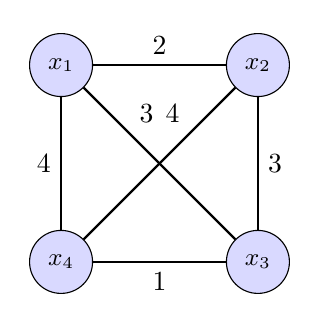
\begin{tikzpicture}[
    node distance=2.5cm,
    point/.style={circle, draw, fill=blue!15, minimum size=8mm, inner sep=0pt, font=\small}
  ]
    \node[point] (x1) {$x_1$};
    \node[point, right of=x1] (x2) {$x_2$};
    \node[point, below of=x2] (x3) {$x_3$};
    \node[point, below of=x1] (x4) {$x_4$};

    \draw[thick] (x1) -- node[above] {$2$} (x2);
    \draw[thick] (x2) -- node[right] {$3$} (x3);
    \draw[thick] (x3) -- node[below] {$1$} (x4);
    \draw[thick] (x4) -- node[left]  {$4$} (x1);
    \draw[thick] (x1) -- node[above right, pos=0.3] {$3$} (x3);
    \draw[thick] (x2) -- node[above left, pos=0.3]  {$4$} (x4);
  \end{tikzpicture}
  \end{center}

  この場合の距離行列は
  \[
    \mathbf{D} =
    \begin{pmatrix}
      0 & 2 & 3 & 4 \\
      2 & 0 & 3 & 4 \\
      3 & 3 & 0 & 1 \\
      4 & 4 & 1 & 0
    \end{pmatrix}
  \]
  である．
\end{example}

\begin{definition}{コーシー列}{cauchy-sequence}
  距離空間 $(X, d)$ における列 $(x_n)_{n \geq 1} \subset X$ が
  \textbf{コーシー列}（Cauchy sequence）であるとは，
  任意の $\varepsilon > 0$ に対してある $N \in \N$ が存在し，
  $n, m \geq N$ ならば $d(x_n, x_m) < \varepsilon$ が成り立つことをいう．
\end{definition}

\begin{definition}{完備距離空間}{complete-metric-space}
  距離空間 $(X, d)$ が\textbf{完備}（complete）であるとは，
  $X$ 上のすべてのコーシー列が $X$ の点に収束することをいう．
  すなわち，$(x_n)_{n \geq 1}$ が $X$ のコーシー列ならば，
  ある $x \in X$ が存在して $\lim_{n \to \infty} d(x_n, x) = 0$ となる．
\end{definition}

\begin{remark}{完備でない距離空間の例}{not-complete}
  有理数全体 $\Q$ にユークリッド距離 $d(x,y) = \abs{x - y}$ を入れた空間 $(\Q, d)$ は完備でない．
  例えば，$\sqrt{2}$ の十進展開を途中で打ち切った有理数列
  $x_1 = 1,\; x_2 = 1.4,\; x_3 = 1.41,\; x_4 = 1.414,\; \ldots$
  は $\Q$ 上のコーシー列であるが，極限 $\sqrt{2} \notin \Q$ であるから
  $\Q$ の中では収束しない．
  $\R$ は $\Q$ をこのような「穴」がないように完備化した空間と見なせる．
\end{remark}

\begin{definition}{コンパクト集合}{compact}
  距離空間 $(X, d)$ の部分集合 $K \subset X$ が\textbf{コンパクト}（compact）であるとは，
  $K$ の任意の点列が $K$ の点に収束する部分列を持つことをいう．
\end{definition}

\begin{example}{$\R^d$ におけるコンパクト集合}{compact-example}
  $\R^d$ の部分集合がコンパクトであることは，
  その集合が\textbf{有界}（ある開球 $B(0, R)$ に含まれる）かつ
  \textbf{閉}であることと同値である（Heine--Borel の定理）．
  例えば閉区間 $[a, b] \subset \R$ はコンパクトであるが，
  開区間 $(a, b)$ は閉でないためコンパクトでなく，
  $\R$ 自身は有界でないためコンパクトでない．
\end{example}

\begin{definition}{可算集合}{countable}
  集合 $A$ が\textbf{可算}（countable）であるとは，
  $A$ から自然数全体 $\N$ への単射が存在することをいう．
  すなわち，$A$ の元を $a_1, a_2, a_3, \ldots$ と番号付けできる．
  有限集合は可算であり，$\N$，$\Z$，$\Q$ は可算である．
  一方，$\R$ は可算でない（非可算である）．
\end{definition}

\begin{definition}{稠密部分集合と可分性}{separable}
  距離空間 $(X, d)$ の部分集合 $D \subset X$ が\textbf{稠密}（dense）であるとは，
  任意の $x \in X$ と任意の $\varepsilon > 0$ に対して，
  ある $y \in D$ が存在して $d(x, y) < \varepsilon$ が成り立つことをいう．
  $X$ が\textbf{可算}な稠密部分集合を持つとき，$X$ は\textbf{可分}（separable）であるという．
\end{definition}

\begin{example}{$\R$ の可分性}{separable-example}
  $\Q$ は $\R$ の稠密部分集合である．
  実際，任意の $x \in \R$ と任意の $\varepsilon > 0$ に対して，
  $\R$ のアルキメデスの性質
  （任意の $\varepsilon > 0$ に対して $n\varepsilon > 1$ となる $n \in \N$ が存在する）
  から $1/n < \varepsilon$ となる $n$ が取れる．
  すると $\abs{x - m/n} < 1/n < \varepsilon$ を満たす整数 $m$ が存在し，
  $q = m/n \in \Q$ が所望の有理数を与える．
  $\Q$ は可算集合であるから（定義~\ref{def:countable}），$\R$ は可分である．

  一方，$\Z$ は $\R$ の稠密部分集合ではない．
  例えば $x = 0.5$，$\varepsilon = 0.1$ に対して
  $\abs{0.5 - n} < 0.1$ を満たす $n \in \Z$ は存在しない．
\end{example}

\begin{definition}{ポーランド空間}{polish-space}
  完備かつ可分な距離空間を\textbf{ポーランド空間}（Polish space）と呼ぶ．
\end{definition}

\begin{proposition}{ポーランド空間の例}{polish-examples}
  以下はいずれもポーランド空間である．
  \begin{enumerate}
    \item $\R^d$（ユークリッド距離）．
    \item 任意のコンパクト距離空間．
    \item 任意の可分バナッハ空間（ノルムから誘導される距離について）．
  \end{enumerate}
\end{proposition}

\begin{proof}
  各場合について，完備性と可分性を確認する．

  \textbf{(1)}
  $\R^d$ の完備性は解析学の基本定理である（コーシー列が収束すること）．
  可分性は，$\Q^d$ が可算稠密部分集合であることから従う
  （例~\ref{ex:separable-example}）．

  \textbf{(2)}
  コンパクト距離空間 $(X, d)$ が完備であることを示す．
  $(x_n)$ を $X$ のコーシー列とする．$X$ はコンパクトであるから，
  収束する部分列 $x_{n_k} \to x \in X$ が存在する．
  コーシー列の部分列が収束するとき，元の列全体も同じ極限に収束する．
  実際，任意の $\varepsilon > 0$ に対して，
  $d(x_n, x_m) < \varepsilon/2$（$n, m \geq N_1$）かつ
  $d(x_{n_k}, x) < \varepsilon/2$（$n_k \geq N_2$）となる $N_1, N_2$ が取れるので，
  $n \geq \max(N_1, N_2)$ に対して $n_k \geq \max(N_1, N_2)$ なる $k$ を選べば
  $d(x_n, x) \leq d(x_n, x_{n_k}) + d(x_{n_k}, x) < \varepsilon$ となる．

  可分性を示す．各 $k \in \N$ に対して，
  $X$ の開被覆 $\{B(x, 1/k) \mid x \in X\}$ を考える
  （$B(x, r)$ は中心 $x$，半径 $r$ の開球）．
  $X$ はコンパクトであるから有限部分被覆
  $X = \bigcup_{i=1}^{N_k} B(x_i^{(k)}, 1/k)$ が存在する．
  $D = \bigcup_{k=1}^{\infty} \{x_1^{(k)}, \ldots, x_{N_k}^{(k)}\}$ とおけば，
  $D$ は可算集合であり，任意の $x \in X$ と任意の $\varepsilon > 0$ に対して
  $1/k < \varepsilon$ なる $k$ を選べば $d(x, x_i^{(k)}) < 1/k < \varepsilon$
  なる $x_i^{(k)} \in D$ が存在するので，$D$ は稠密である．

  \textbf{(3)}
  バナッハ空間はノルムから誘導される距離に関して定義により完備である．
  可分性は仮定として課されている．
\end{proof}

ポーランド空間を導入する理由は，この空間上で確率測度の集合に良いコンパクト性が成り立ち，
最適輸送問題の解の存在が保証されるためである．
詳細は確率測度を定義した後，\ref{subsec:prokhorov}~節で述べる．

%% --- 1.3.2 可測空間とボレル σ-代数 ---
\subsection{可測空間とボレル集合族}
\label{subsec:measurable-space}

測度を定義するためには，まず「測定可能な」集合の族を定める必要がある．
その準備として，距離空間における開集合と閉集合を定義する．

\begin{definition}{開球}{open-ball}
  距離空間 $(X, d)$ において，点 $x \in X$ と実数 $r > 0$ に対して，
  \textbf{開球}（open ball）を
  $B(x, r) \defeq \{y \in X \mid d(x, y) < r\}$
  で定義する．
\end{definition}

\begin{definition}{開集合と閉集合}{open-closed}
  距離空間 $(X, d)$ の部分集合 $U \subset X$ が\textbf{開集合}（open set）であるとは，
  任意の $x \in U$ に対してある $r > 0$ が存在して
  $B(x, r) \subset U$ が成り立つことをいう．
  すなわち，$U$ の各点のまわりに $U$ に含まれる開球が取れる．

  部分集合 $F \subset X$ が\textbf{閉集合}（closed set）であるとは，
  その補集合 $F^c = X \setminus F$ が開集合であることをいう．
  同値な特徴づけとして，$F$ が閉集合であることは，
  $F$ の点列の極限が常に $F$ に属すること
  （すなわち $x_n \in F$，$x_n \to x$ ならば $x \in F$）と同値である．
\end{definition}

\begin{example}{$\R$ における開集合と閉集合}{open-closed-example}
  $\R$ 上の通常の距離 $d(x,y) = \abs{x-y}$ を考える．
  \begin{itemize}
    \item 開区間 $(a, b) = \{x \in \R \mid a < x < b\}$ は開集合である．
      任意の $x \in (a, b)$ に対して $r = \min(x - a, b - x) > 0$ と取れば
      $B(x, r) \subset (a, b)$ となる．
    \item 閉区間 $[a, b] = \{x \in \R \mid a \leq x \leq b\}$ は閉集合である．
      $[a, b]$ の点列 $x_n \to x$ ならば $a \leq x \leq b$ であるから $x \in [a, b]$ となる．
    \item 半開区間 $[a, b)$ は開集合でも閉集合でもない．
      点 $a$ のまわりに $[a, b)$ に含まれる開球は取れず（$a - r < a$ となる点を含めない），
      また列 $b - 1/n \to b$ に対して $b \notin [a, b)$ であるから閉でもない．
  \end{itemize}
\end{example}

\begin{definition}{$\sigma$-代数}{sigma-algebra}
  集合 $X$ の部分集合族 $\Bb \subset 2^X$ が\textbf{$\sigma$-代数}
  （$\sigma$-algebra）であるとは，以下の3条件を満たすことをいう：
  \begin{enumerate}
    \item $X \in \Bb$．
    \item $A \in \Bb$ ならば $A^c = X \setminus A \in \Bb$（補集合で閉じている）．
    \item $A_1, A_2, \ldots \in \Bb$ ならば
      $\bigcup_{k=1}^{\infty} A_k \in \Bb$（可算合併で閉じている）．
  \end{enumerate}
  組 $(X, \Bb)$ を\textbf{可測空間}（measurable space）と呼ぶ．
\end{definition}

\begin{definition}{ボレル $\sigma$-代数}{borel}
  距離空間 $(X, d)$ に対して，$X$ の\textbf{すべての開集合}を含む最小の $\sigma$-代数を
  \textbf{ボレル $\sigma$-代数}（Borel $\sigma$-algebra）と呼び，$\Bb(X)$ と記す．
  $\Bb(X)$ の元を\textbf{ボレル集合}（Borel set）と呼ぶ．
\end{definition}

\begin{remark}{}{borel-remark}
  ボレル $\sigma$-代数は開集合・閉集合を含み，
  それらの可算回の合併・交差・補集合操作で得られるすべての集合を含む．
  $\R^d$ のボレル $\sigma$-代数 $\Bb(\R^d)$ は，
  距離空間上の確率論や測度論の標準的な枠組みとなる．
  以降，距離空間上の測度は常にボレル $\sigma$-代数に関して定義されるものとする．
\end{remark}

%% --- 1.3.4 測度と確率測度 ---
\subsection{測度と確率測度}
\label{subsec:measures}

\begin{definition}{測度}{measure}
  可測空間 $(X, \Bb)$ 上の\textbf{測度}（measure）とは，
  関数 $\mu \colon \Bb \to [0, \infty]$ であって，以下を満たすものをいう：
  \begin{enumerate}
    \item $\mu(\emptyset) = 0$．
    \item \textbf{可算加法性}：互いに素な列 $A_1, A_2, \ldots \in \Bb$
      に対して $\mu\!\left(\bigcup_{k=1}^{\infty} A_k\right) = \sum_{k=1}^{\infty} \mu(A_k)$．
  \end{enumerate}
\end{definition}

\begin{definition}{確率測度}{probability-measure}
  距離空間 $X$ 上の\textbf{確率測度}（probability measure）とは，
  ボレル $\sigma$-代数 $\Bb(X)$ 上の測度 $\mu$ であって $\mu(X) = 1$ を満たすものをいう．
  $X$ 上のすべての確率測度の集合を
  \[
    \Mm_+^1(X) \defeq \left\{ \mu \in \Mm_+(X) \;\middle|\; \mu(X) = 1 \right\}
  \]
  と記す．ここで $\Mm_+(X)$ は $X$ 上のすべての非負ボレル測度の集合である．
\end{definition}

\begin{remark}{測度の直感的理解}{measure-intuition}
  測度とは，集合の各部分に「大きさ」や「質量」を割り当てる関数である．
  確率測度は全体の質量が1に正規化されたものであり，「確率分布」と同義に用いられる．
  砂山の比喩を使えば，確率測度は「各領域にどれだけの砂があるか」を記述する．
\end{remark}

\begin{definition}{測度の台}{support}
  距離空間 $X$ 上の測度 $\mu$ の\textbf{台}（support）とは，
  \[
    \supp(\mu) \defeq \left\{ x \in X \;\middle|\;
    \text{$x$ を含むすべての開集合 $U$ に対して } \mu(U) > 0 \right\}
  \]
  で定義される $X$ の部分集合をいう．
\end{definition}

$\supp(\mu)$ は閉集合である．
実際，補集合
\[
  \supp(\mu)^c = \{x \in X \mid x \in U,\; \mu(U) = 0 \text{ なる開集合 } U \text{ が存在する}\}
\]
が開集合であることを示せばよい．
$x \in \supp(\mu)^c$ ならば $x \in U$，$\mu(U) = 0$ なる開集合 $U$ が存在する．
任意の $y \in U$ に対して，$U$ は $y$ の開近傍でもあり $\mu(U) = 0$ であるから，
$y \in \supp(\mu)^c$ となる．よって $U \subset \supp(\mu)^c$ であり，
$\supp(\mu)^c$ は開集合である．

\begin{definition}{ディラック測度}{dirac}
  距離空間 $X$ の点 $x \in X$ に対して，\textbf{ディラック測度}（Dirac measure）
  $\delta_x$ を
  \[
    \delta_x(A) \defeq
    \begin{cases}
      1 & x \in A, \\
      0 & x \notin A
    \end{cases}
    \qquad (A \in \Bb(X))
  \]
  で定義する．すなわち，$\delta_x$ は点 $x$ に全質量を集中させた確率測度である．
  ディラック測度に対する積分は
  $\int_X f(y) \, \d\delta_x(y) = f(x)$
  で与えられる．
\end{definition}

%% --- 1.3.5 確率測度のコンパクト性と Prokhorov の定理 ---
\subsection{確率測度のコンパクト性と Prokhorov の定理}
\label{subsec:prokhorov}

最適輸送の Kantorovich 問題（\ref{sec:kantorovich-overview}~節で定式化）では，
カップリング測度の集合の上でコストの下限を取る．
この下限が実際に達成される（最適解が存在する）ためには，
カップリングの集合がある種のコンパクト性を持つ必要がある．

ポーランド空間上では，確率測度の集合のコンパクト性を
「緊密性」という条件で特徴づけることができる．
これが Prokhorov の定理であり，
ポーランド空間を導入する根本的な理由である．
完備性がなければ極限測度が空間上の測度とならない可能性があり，
可分性がなければ以下の同値関係が成り立たない．

まず，確率測度の列が「収束する」とはどういう意味かを定める．
直感的には，測度 $\mu_n$ が $\mu$ に近づくとは，
任意の連続関数 $f$ に対して $f$ の $\mu_n$ による積分が $f$ の $\mu$ による積分に近づくことをいう．

\begin{definition}{有界関数}{bounded-function}
  距離空間 $X$ 上の関数 $f \colon X \to \R$ が\textbf{有界}（bounded）であるとは，
  ある定数 $M \geq 0$ が存在して，すべての $x \in X$ に対して $\abs{f(x)} \leq M$
  が成り立つことをいう．
\end{definition}

\begin{definition}{確率測度の弱収束}{weak-convergence}
  ポーランド空間 $X$ 上の確率測度の列 $(\mu_n)_{n \geq 1}$ が
  確率測度 $\mu$ に\textbf{弱収束}（weakly converge）するとは，
  すべての有界連続関数 $f \colon X \to \R$ に対して
  \[
    \lim_{n \to \infty} \int_X f \, \d\mu_n = \int_X f \, \d\mu
  \]
  が成り立つことをいう．
\end{definition}

弱収束する部分列を取るためには，
測度の質量が無限遠に「逃げない」ことが必要である．
例えば，$\R$ 上のディラック測度の列 $\mu_n = \delta_n$
（点 $n$ に全質量を集中させた測度）を考える．

\begin{center}
\begin{tikzpicture}[scale=0.85]
  % --- 緊密でない例（上段） ---
  \node[left, font=\small\bfseries] at (-1, 1.5) {緊密でない：};
  \draw[thick, ->] (-0.5, 0) -- (10.5, 0);
  % mu_1
  \draw[thick, blue] (1, 0) -- (1, 1.0);
  \fill[blue] (1, 1.0) circle (2pt);
  \node[below, font=\small] at (1, -0.1) {$1$};
  \node[above, blue, font=\small] at (1, 1.1) {$\mu_1$};
  % mu_2
  \draw[thick, blue] (3, 0) -- (3, 1.0);
  \fill[blue] (3, 1.0) circle (2pt);
  \node[below, font=\small] at (3, -0.1) {$2$};
  \node[above, blue, font=\small] at (3, 1.1) {$\mu_2$};
  % mu_3
  \draw[thick, blue] (5, 0) -- (5, 1.0);
  \fill[blue] (5, 1.0) circle (2pt);
  \node[below, font=\small] at (5, -0.1) {$3$};
  \node[above, blue, font=\small] at (5, 1.1) {$\mu_3$};
  % mu_4
  \draw[thick, blue] (7, 0) -- (7, 1.0);
  \fill[blue] (7, 1.0) circle (2pt);
  \node[below, font=\small] at (7, -0.1) {$4$};
  \node[above, blue, font=\small] at (7, 1.1) {$\mu_4$};
  % dots
  \node at (9, 0.5) {$\cdots$};
  % arrow
  \draw[->, thick, gray, dashed] (1.5, -0.6) -- (8.5, -0.6);
  \node[below, gray, font=\small] at (5, -0.7) {質量が右へ逃げていく};

  % --- 緊密な例（下段） ---
  \begin{scope}[yshift=-3.8cm]
    \node[left, font=\small\bfseries] at (-1, 1.5) {緊密：};
    \draw[thick, ->] (-0.5, 0) -- (10.5, 0);
    % compact set K (bracket below axis)
    \draw[thick, red!70!black, decorate, decoration={brace, mirror, amplitude=5pt}]
      (0.8, -0.4) -- (6.2, -0.4)
      node[midway, below=6pt, red!70!black, font=\small] {コンパクト集合 $K$};
    % mu_1
    \draw[thick, blue] (1.5, 0) -- (1.5, 0.8);
    \fill[blue] (1.5, 0.8) circle (2pt);
    \node[above, blue, font=\small] at (1.5, 0.9) {$\mu_1$};
    % mu_4
    \draw[thick, blue] (2.3, 0) -- (2.3, 0.9);
    \fill[blue] (2.3, 0.9) circle (2pt);
    \node[above, blue, font=\small] at (2.3, 1.0) {$\mu_4$};
    % mu_2
    \draw[thick, blue] (3.5, 0) -- (3.5, 1.0);
    \fill[blue] (3.5, 1.0) circle (2pt);
    \node[above, blue, font=\small] at (3.5, 1.1) {$\mu_2$};
    % mu_3
    \draw[thick, blue] (5, 0) -- (5, 0.6);
    \fill[blue] (5, 0.6) circle (2pt);
    \node[above, blue, font=\small] at (5, 0.7) {$\mu_3$};
    % dots
    \node at (5.8, 0.5) {$\cdots$};
  \end{scope}
\end{tikzpicture}
\end{center}

上段は緊密でない場合：各 $\mu_n = \delta_n$ の質量が際限なく移動し，
どのコンパクト集合 $K$ を取っても，十分大きな $n$ で $\mu_n(K) = 0$ となるため，
収束する部分列が存在しない．
下段は緊密な場合：すべての $\mu_n$ の質量が共通のコンパクト集合 $K$ にほぼ収まっており，
収束する部分列を取ることができる．
緊密性はこのような状況を排除する条件である．

\begin{definition}{緊密性}{tightness}
  ポーランド空間 $X$ 上の確率測度の集合 $\Pi \subset \Mm_+^1(X)$ が
  \textbf{緊密}（tight）であるとは，
  任意の $\varepsilon > 0$ に対してコンパクト集合 $K \subset X$ が存在し，
  すべての $\mu \in \Pi$ に対して $\mu(K) \geq 1 - \varepsilon$ が成り立つことをいう．
  すなわち，$\Pi$ に属するすべての測度の質量が，共通のコンパクト集合にほぼ集中している．
\end{definition}

\begin{definition}{相対コンパクト性}{relatively-compact}
  距離空間の部分集合 $S$ が\textbf{相対コンパクト}（relatively compact）であるとは，
  $S$ の任意の列が収束する部分列を持つことをいう．
\end{definition}

コンパクト集合の定義（定義~\ref{def:compact}）では
部分列の極限が元の集合に属することを要求するが，
相対コンパクトでは極限が $S$ の外にあってもよい．
$\R^d$ において「有界な列は収束部分列を持つ」（Bolzano--Weierstrass の定理）は，
有界集合が相対コンパクトであることの主張に他ならない．

\begin{theorem}{Prokhorov の定理}{prokhorov}
  ポーランド空間 $X$ 上の確率測度の集合 $\Pi \subset \Mm_+^1(X)$ に対して，
  以下は同値である：
  \begin{enumerate}
    \item $\Pi$ は緊密である．
    \item $\Pi$ は弱収束に関して相対コンパクトである．
  \end{enumerate}
\end{theorem}

\begin{proof}
  \textbf{(1) $\Rightarrow$ (2)：緊密ならば相対コンパクト．}

  $\Pi$ が緊密であるとし，$(\mu_n)_{n \geq 1}$ を $\Pi$ の任意の列とする．
  弱収束する部分列の存在を示す．

  \textit{ステップ1：対角線論法．}
  $X$ は可分であるから，$X$ 上の有界連続関数の中から
  可算族 $\{f_k\}_{k \geq 1}$ であって弱収束を決定するものが取れる
  （すなわち，すべての $k$ で $\int f_k \, \d\mu_n \to \int f_k \, \d\mu$
  が成り立てば $\mu_n$ は $\mu$ に弱収束する）．
  各 $k$ に対して，数列 $(\int f_k \, \d\mu_n)_{n \geq 1}$ は有界であるから，
  Bolzano--Weierstrass の定理により収束する部分列が取れる．
  対角線論法を適用すると，ある部分列 $(\mu_{n_j})_{j \geq 1}$ が存在して，
  すべての $k$ に対して $\lim_{j \to \infty} \int f_k \, \d\mu_{n_j}$ が存在する．

  \textit{ステップ2：極限測度の構成．}
  写像 $\Lambda(f_k) \defeq \lim_{j \to \infty} \int f_k \, \d\mu_{n_j}$
  は有界連続関数上の正値線形汎関数に拡張される．
  Riesz の表現定理により，ある非負測度 $\mu$ が存在して
  $\Lambda(f) = \int f \, \d\mu$ が成り立つ．

  \textit{ステップ3：$\mu$ が確率測度であること．}
  ここで緊密性が本質的に用いられる．
  任意の $\varepsilon > 0$ に対して，緊密性からコンパクト集合 $K$ が存在し，
  すべての $n$ で $\mu_n(K) \geq 1 - \varepsilon$ が成り立つ．
  コンパクト集合は閉集合であるから，弱収束の性質（Portmanteau の定理）より
  \[
    \mu(K) \geq \limsup_{j \to \infty} \mu_{n_j}(K) \geq 1 - \varepsilon.
  \]
  $\varepsilon > 0$ は任意であったから $\mu(X) \geq \mu(K) \geq 1 - \varepsilon$ より
  $\mu(X) = 1$，すなわち $\mu$ は確率測度である．

  \medskip
  \textbf{(2) $\Rightarrow$ (1)：相対コンパクトならば緊密．}

  対偶を示す．$\Pi$ が緊密でないと仮定する．
  すなわち，ある $\varepsilon_0 > 0$ が存在して，
  任意のコンパクト集合 $K \subset X$ に対して
  ある $\mu \in \Pi$ が $\mu(K) < 1 - \varepsilon_0$ を満たす．

  $X$ は可分であるから稠密な可算集合 $\{x_k\}_{k \geq 1}$ が取れる．
  各 $n \in \N$ に対して，コンパクト集合
  \[
    K_{n,N} \defeq \bigcup_{k=1}^N \overline{B(x_k, 1/n)}
  \]
  を考える（有限個の閉球の合併であり，$X$ の完備性から閉かつ全有界なのでコンパクト）．
  $\bigcup_{N=1}^{\infty} K_{n,N} = X$ であるから，
  任意の確率測度 $\mu$ に対して $\mu(K_{n,N}) \to 1$ （$N \to \infty$）が成り立つ．

  しかし，$\Pi$ が緊密でないことから，
  任意のコンパクト集合 $K$ に対して $\mu_K(K) < 1 - \varepsilon_0$ なる
  $\mu_K \in \Pi$ が取れる．
  コンパクト集合を $K_1 \subset K_2 \subset \cdots$ と
  $\bigcup_m K_m = X$ なる増大列に取り
  （例えば $K_m = \bigcap_{n=1}^m K_{n, N_n}$ を適切な $N_n$ で構成する），
  各 $m$ に対して $\mu_m \in \Pi$ を $\mu_m(K_m) < 1 - \varepsilon_0$ なるように選ぶ．

  この列 $(\mu_m)$ が弱収束する部分列を持たないことを示す．
  仮に部分列 $\mu_{m_j} \to \mu$ が弱収束するとする．
  任意の固定された $\ell$ に対して，$m_j \geq \ell$ ならば $K_\ell \subset K_{m_j}$ であるから
  $\mu_{m_j}(K_\ell) \leq \mu_{m_j}(K_{m_j}) < 1 - \varepsilon_0$ が成り立つ．
  $K_\ell$ は閉集合であるから，Portmanteau の定理より
  \[
    \mu(K_\ell) \geq \limsup_{j \to \infty} \mu_{m_j}(K_\ell) \geq 0.
  \]
  一方，上の不等式から各 $\mu_{m_j}(K_\ell) < 1 - \varepsilon_0$ であるから
  $\limsup_{j} \mu_{m_j}(K_\ell) \leq 1 - \varepsilon_0$ となり，
  \[
    \mu(K_\ell) \leq 1 - \varepsilon_0 \quad (\forall\, \ell).
  \]
  $\ell \to \infty$ で $K_\ell \uparrow X$ であるから
  $\mu(X) = \lim_\ell \mu(K_\ell) \leq 1 - \varepsilon_0 < 1$ となる．
  しかし $\mu$ は弱極限であるから $\mu(X) = 1$ でなければならず，矛盾する．

  よって $(\mu_m)$ は弱収束する部分列を持たず，$\Pi$ は相対コンパクトでない．
\end{proof}

%% --- 1.3.6 確率単体 ---
\subsection{確率単体}
\label{subsec:simplex}

有限集合 $\{1, \ldots, n\}$ 上の確率測度は，
非負の重みベクトル $\mathbf{a} = (a_1, \ldots, a_n)$ で $\sum_i a_i = 1$ を満たすものと
同一視できる．このようなベクトルの全体が確率単体である．

\begin{definition}{確率単体}{simplex}
  $n$ 次元の\textbf{確率単体}（probability simplex）とは，
  $\R^n$ の部分集合
  \[
    \simplex_n \defeq
    \left\{ \mathbf{a} \in \R_+^n \;\middle|\; \sum_{i=1}^n a_i = 1 \right\}
  \]
  をいう．$\simplex_n$ の元を\textbf{確率ベクトル}（probability vector）
  または\textbf{ヒストグラム}（histogram）と呼ぶ．
\end{definition}

\begin{remark}{}{simplex-properties}
  $\simplex_n$ は $\R^n$ の\textbf{凸}かつ\textbf{コンパクト}な部分集合である．
  その端点（extreme points）は標準基底ベクトル $e_1, \ldots, e_n$ であり，
  $\simplex_n$ はこれらの凸包に等しい：
  $\simplex_n = \operatorname{conv}(e_1, \ldots, e_n)$．
\end{remark}

\begin{example}{低次元の確率単体}{simplex-low-dim}
  \begin{itemize}
    \item $n = 2$ のとき，$\simplex_2 = \{(a_1, a_2) \in \R_+^2 \mid a_1 + a_2 = 1\}$
      は $(1, 0)$ と $(0, 1)$ を結ぶ線分である．
    \item $n = 3$ のとき，$\simplex_3$ は $\R^3$ 内の三角形であり，
      頂点 $(1,0,0)$, $(0,1,0)$, $(0,0,1)$ を持つ．
  \end{itemize}

  \begin{center}
  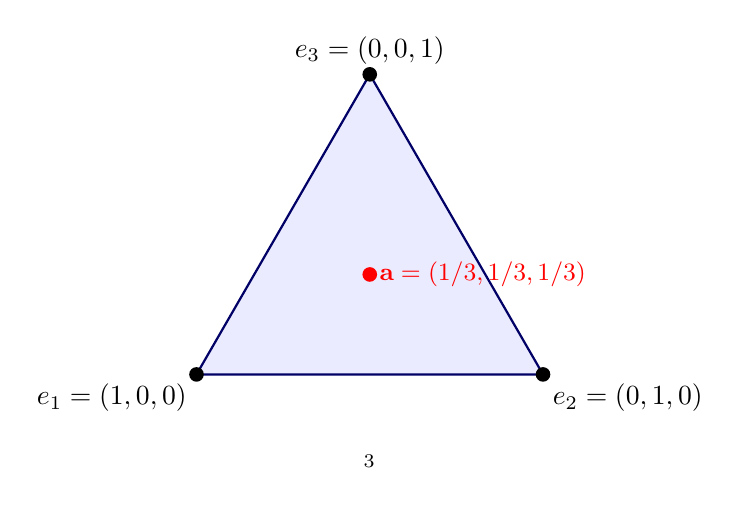
\begin{tikzpicture}[scale=2.2]
    % 2-simplex (triangle) in 2D projection
    \coordinate (A) at (0, 0);
    \coordinate (B) at (2, 0);
    \coordinate (C) at (1, 1.732);

    \fill[blue!8] (A) -- (B) -- (C) -- cycle;
    \draw[blue!40!black, thick] (A) -- (B) -- (C) -- cycle;

    \fill (A) circle (1.2pt) node[below left] {$e_1 = (1,0,0)$};
    \fill (B) circle (1.2pt) node[below right] {$e_2 = (0,1,0)$};
    \fill (C) circle (1.2pt) node[above] {$e_3 = (0,0,1)$};

    % sample point
    \coordinate (P) at (1, 0.577);
    \fill[red] (P) circle (1.2pt) node[right] {\small $\mathbf{a} = (1/3, 1/3, 1/3)$};

    \node at (1, -0.5) {$\simplex_3$};
  \end{tikzpicture}
  \end{center}
\end{example}

%% --- 1.3.7 離散測度 ---
\subsection{離散測度}
\label{subsec:discrete-measures}

ディラック測度（定義~\ref{def:dirac}）を用いて，有限個の点に質量を持つ測度を構成できる．

\begin{remark}{}{dirac-integration}
  離散測度に対する積分を和に帰着させる際の基本は，
  ディラック測度に対する積分の性質
  $\int_X f(y) \, \d\delta_x(y) = f(x)$（定義~\ref{def:dirac}）である．
\end{remark}

\begin{definition}{離散測度}{discrete-measure}
  距離空間 $X$ 上の\textbf{離散測度}（discrete measure）とは，
  有限個の点 $x_1, \ldots, x_n \in X$ と非負の重み $a_1, \ldots, a_n > 0$ に対して
  \[
    \alpha = \sum_{i=1}^n a_i \, \delta_{x_i}
  \]
  の形で表される測度をいう．
  さらに $\mathbf{a} = (a_1, \ldots, a_n) \in \simplex_n$ が成り立つとき，
  $\alpha$ は\textbf{離散確率測度}（discrete probability measure）と呼ばれる．
\end{definition}

\begin{remark}{ヒストグラムと離散測度の関係}{histogram-vs-discrete}
  ヒストグラム $\mathbf{a} \in \simplex_n$ は，ビンの位置が固定された場合の確率ベクトルである．
  離散測度 $\alpha = \sum_i a_i \delta_{x_i}$ は，
  確率ベクトル $\mathbf{a}$ に加えて，各ビンの\textbf{位置} $(x_1, \ldots, x_n)$ の情報も持つ．
  ヒストグラムは「重みのみ」を記述し，離散測度は「重みと位置の両方」を記述する．
  この区別は，特に異なる台を持つ離散測度を比較する際に本質的な意味を持つ．
\end{remark}

\begin{example}{経験分布}{empirical}
  データ点 $x_1, \ldots, x_n \in X$ が何らかの確率分布から独立にサンプルされたとき，
  \textbf{経験分布}（empirical distribution）
  \[
    \hat{\mu}_n = \frac{1}{n} \sum_{i=1}^n \delta_{x_i}
  \]
  は，データの分布を近似する離散確率測度である．
  大数の法則により，$n \to \infty$ で $\hat{\mu}_n$ は真の分布に弱収束する．
  経験分布は最適輸送の応用（特に統計的推定）において重要な対象である．
\end{example}

%% --- 1.3.6 測度の密度 ---
\subsection{測度の密度}
\label{subsec:density}

離散測度に対する対極として，ルベーグ測度に関して連続的な密度を持つ測度がある．

\begin{definition}{ルベーグ測度に関する密度}{lebesgue-density}
  $X = \R^d$ 上の測度 $\alpha$ が
  ルベーグ測度に関して\textbf{密度}（density）$\rho_\alpha$ を持つとは，
  非負可測関数 $\rho_\alpha \colon \R^d \to [0, \infty)$ が存在して，
  すべてのボレル集合 $A \in \Bb(\R^d)$ に対して
  \[
    \alpha(A) = \int_A \rho_\alpha(x) \, \d x
  \]
  が成り立つことをいう．ここで右辺はルベーグ積分である．
  このとき $\rho_\alpha = \frac{\d\alpha}{\d x}$ と記す．
  $\alpha$ が確率測度であるためには，$\int_{\R^d} \rho_\alpha(x) \, \d x = 1$ が必要十分である．
\end{definition}

\begin{definition}{ラドン--ニコディム導関数}{radon-nikodym}
  より一般に，測度 $\alpha$ が測度 $\beta$ に関して\textbf{絶対連続}
  （absolutely continuous; $\alpha \ll \beta$ と記す）であるとは，
  $\beta(A) = 0$ ならば $\alpha(A) = 0$ が成り立つことをいう．
  このとき，ラドン--ニコディムの定理により，
  $\beta$-可測関数 $\frac{\d\alpha}{\d\beta} \geq 0$ が $\beta$-a.e.\ に一意的に存在して，
  \[
    \alpha(A) = \int_A \frac{\d\alpha}{\d\beta}(x) \, \d\beta(x)
    \qquad (\forall\, A \in \Bb(X))
  \]
  が成り立つ．この関数 $\frac{\d\alpha}{\d\beta}$ を
  $\alpha$ の $\beta$ に関する\textbf{ラドン--ニコディム導関数}
  （Radon--Nikodym derivative）または\textbf{相対密度}と呼ぶ．
\end{definition}

\begin{remark}{測度の3つの類型}{three-types}
  最適輸送の理論では，主に以下の3種類の測度を扱う：
  \begin{enumerate}
    \item \textbf{ヒストグラム}：$\mathbf{a} \in \simplex_n$（有限次元の確率ベクトル）．
      ビンの位置は固定されており，最も単純な設定である．
    \item \textbf{離散測度}：$\alpha = \sum_i a_i \delta_{x_i}$（有限個の点に台を持つ測度）．
      重みと位置の両方が自由度を持つ．
    \item \textbf{連続測度}：$\d\alpha(x) = \rho_\alpha(x) \, \d x$
      （ルベーグ測度に関して密度を持つ測度）．
      最も一般的であるが，計算上は最も扱いが難しい．
  \end{enumerate}
  本書では，主にヒストグラムと離散測度を扱い，
  必要に応じて連続測度への拡張にも触れる．
\end{remark}

%% --- 1.3.7 コスト関数 ---
\subsection{コスト関数}
\label{subsec:cost-function}

最適輸送の目的関数を定めるのがコスト関数である．

\begin{definition}{コスト関数}{cost-function}
  空間 $\X$ と $\Y$ に対して，\textbf{コスト関数}（cost function）とは，
  可測関数
  \[
    c \colon \X \times \Y \to \R_+ \cup \{+\infty\}
  \]
  をいう．$c(x, y)$ は，点 $x \in \X$ から点 $y \in \Y$ へ単位質量を輸送するコストを表す．
\end{definition}

\begin{example}{典型的なコスト関数}{cost-examples}
  $(X, d)$ を距離空間とし，$\X = \Y = X$ とする．
  \begin{enumerate}
    \item \textbf{距離コスト}：$c(x, y) = d(x, y)$．
      $p$-Wasserstein 距離（$p=1$）に対応する．
    \item \textbf{二乗距離コスト}：$c(x, y) = d(x, y)^2$．
      最もよく研究されているケースであり，Brenier の定理の仮定となる．
      特に $X = \R^d$ では $c(x,y) = \norm{x-y}_2^2$ である．
    \item \textbf{$p$ 乗距離コスト}：$c(x, y) = d(x, y)^p$（$p \geq 1$）．
      $p$-Wasserstein 距離を導く．
    \item \textbf{離散コスト行列}：
      点集合 $x_1, \ldots, x_n \in \X$ と $y_1, \ldots, y_m \in \Y$ が固定されているとき，
      $n \times m$ 行列 $\mathbf{C}$ を $C_{i,j} = c(x_i, y_j)$ で定義する．
      これを\textbf{コスト行列}（cost matrix）と呼ぶ．
  \end{enumerate}
\end{example}

%% ============================================================
%%  1.4 Monge 問題の概要
%% ============================================================
\section{Monge 問題の概要}
\label{sec:monge-overview}

最適輸送の出発点は，Monge (1781) による次の問題である：
ソース分布 $\alpha$ をターゲット分布 $\beta$ に「移す」写像 $T$ のうち，
総輸送コストを最小にするものを求めよ．
この問題を正確に述べるためには，写像による測度の「移動」を定義する必要がある．

\begin{definition}{押し出し（push-forward）}{pushforward}
  $(X, \Bb(X))$ と $(Y, \Bb(Y))$ を可測空間とし，
  $T \colon X \to Y$ を可測写像とする．
  測度 $\alpha \in \Mm_+(X)$ の $T$ による\textbf{押し出し}
  $T\pushforward \alpha \in \Mm_+(Y)$ を
  \[
    (T\pushforward \alpha)(B) \defeq \alpha(T^{-1}(B))
    \qquad (\forall\, B \in \Bb(Y))
  \]
  で定義する．ここで $T^{-1}(B) = \{x \in X \mid T(x) \in B\}$ は $B$ の逆像である．
\end{definition}

\begin{remark}{}{pushforward-integration}
  押し出しの定義を積分の言葉で述べると，
  すべての可測関数 $h \colon Y \to \R$ に対して
  \[
    \int_Y h(y) \, \d(T\pushforward \alpha)(y) = \int_X h(T(x)) \, \d\alpha(x)
  \]
  が成り立つ．離散測度 $\alpha = \sum_i a_i \delta_{x_i}$ に対しては，
  \[
    T\pushforward \alpha = \sum_{i=1}^n a_i \, \delta_{T(x_i)}
  \]
  となる．すなわち，押し出しは各点 $x_i$ の位置を $T(x_i)$ に移し，重み $a_i$ は保存する操作である．
\end{remark}

以上を用いて，Monge 問題を定式化する．

\begin{setting}{Monge 問題}{monge}
  ソース空間 $\X$ 上の確率測度 $\alpha \in \Mm_+^1(\X)$，
  ターゲット空間 $\Y$ 上の確率測度 $\beta \in \Mm_+^1(\Y)$，
  およびコスト関数 $c \colon \X \times \Y \to \R_+$ が与えられたとき，
  \textbf{Monge 問題}とは次の最適化問題をいう：
  \[
    \inf_{\substack{T \colon \X \to \Y \\ T\pushforward \alpha = \beta}}
    \int_{\X} c(x, T(x)) \, \d\alpha(x).
  \]
  ここで最適化は，$T\pushforward \alpha = \beta$ を満たすすべての可測写像 $T$ にわたって行う．
  条件 $T\pushforward \alpha = \beta$ は，写像 $T$ が
  ソースの質量分布をターゲットの質量分布に正確に移すことを要求する．
\end{setting}

Monge 問題には，以下の本質的な困難がある．

\begin{remark}{Monge 問題の困難}{monge-difficulty}
  \begin{enumerate}
    \item \textbf{非凸性}：
      実行可能集合 $\{T \colon T\pushforward \alpha = \beta\}$ は一般に\textbf{凸でない}．
      すなわち，2つの実行可能な写像 $T_1, T_2$ に対して，
      その凸結合 $(1-t)T_1 + tT_2$ は一般に実行可能でない
      （押し出し条件は写像に関して非線形だからである）．
      このため，標準的な凸最適化の手法が直接は適用できない．

    \item \textbf{解の非存在}：
      以下の例~\ref{ex:monge-nonexistence} に示すように，
      実行可能な写像 $T$ が\textbf{存在しない}場合がある．
      特に，ソース測度がターゲット測度より「粗い」
      （少数の点に質量が集中している）場合に，質量を分割できないという制約が障害となる．
  \end{enumerate}
\end{remark}

\begin{example}{Monge 写像が存在しない場合}{monge-nonexistence}
  $\X = \Y = \R$ 上で，ソース測度 $\alpha = \delta_0$（原点に全質量を集中），
  ターゲット測度 $\beta = \frac{1}{2}\delta_{-1} + \frac{1}{2}\delta_1$
  （$-1$ と $1$ に半分ずつ質量を配置）を考える．

  $T\pushforward \alpha = \beta$ を満たす写像 $T \colon \R \to \R$ が存在すると仮定する．
  $\alpha = \delta_0$ であるから，
  $T\pushforward \delta_0 = \delta_{T(0)}$ となる．
  しかし $\delta_{T(0)}$ は1点に集中した測度であり，
  $\beta = \frac{1}{2}\delta_{-1} + \frac{1}{2}\delta_1$ は2点に質量を持つ．
  よって $\delta_{T(0)} \neq \beta$ であり，矛盾する．

  \begin{center}
  \begin{tikzpicture}[scale=1.1]
    % Source
    \draw[->] (-2, 0) -- (2, 0);
    \draw[thick, blue] (0, 0) -- (0, 1.2);
    \fill[blue] (0, 1.2) circle (2pt);
    \node[below] at (0, -0.1) {$0$};
    \node[above, blue] at (0, 1.35) {$\alpha = \delta_0$};

    % Arrow
    \draw[->, thick, dashed, gray] (2.5, 0.6) -- (3.5, 0.6);
    \node[above, gray] at (3, 0.6) {$T\, ?$};

    % Target
    \begin{scope}[xshift=5.5cm]
      \draw[->] (-2, 0) -- (2, 0);
      \draw[thick, red] (-1, 0) -- (-1, 0.6);
      \fill[red] (-1, 0.6) circle (2pt);
      \draw[thick, red] (1, 0) -- (1, 0.6);
      \fill[red] (1, 0.6) circle (2pt);
      \node[below] at (-1, -0.1) {$-1$};
      \node[below] at (1, -0.1) {$1$};
      \node[above, red] at (0, 0.8) {$\beta = \tfrac{1}{2}\delta_{-1} + \tfrac{1}{2}\delta_1$};
    \end{scope}
  \end{tikzpicture}
  \end{center}

  この例は，Monge の定式化では質量の「分割」が許されないために
  解が存在しないことを端的に示している．
  Kantorovich の緩和（次節）は，まさにこの困難を解消するものである．
\end{example}

%% ============================================================
%%  1.5 Kantorovich 緩和の概要
%% ============================================================
\section{Kantorovich 緩和の概要}
\label{sec:kantorovich-overview}

Kantorovich (1942) の革命的なアイデアは，
Monge の決定論的な輸送写像 $T$ を\textbf{確率的な輸送計画}に置き換えることである．
すなわち，各点 $x$ の質量を\textbf{1つの行き先に集中させる}代わりに，
\textbf{複数の行き先に分割して}送ることを許す．
この確率的な輸送計画は，$\X \times \Y$ 上の結合測度（カップリング）として定式化される．

\begin{definition}{カップリング}{coupling}
  確率測度 $\alpha \in \Mm_+^1(\X)$ と $\beta \in \Mm_+^1(\Y)$ に対して，
  $\alpha$ と $\beta$ の\textbf{カップリング}（coupling）の集合を
  \[
    \Couplings(\alpha, \beta) \defeq
    \left\{ \pi \in \Mm_+^1(\X \times \Y) \;\middle|\;
    (P_\X)\pushforward \pi = \alpha, \;
    (P_\Y)\pushforward \pi = \beta \right\}
  \]
  で定義する．ここで $P_\X(x, y) = x$，$P_\Y(x, y) = y$ はそれぞれ
  第1成分・第2成分への射影である．
  すなわち，$\pi$ の\textbf{周辺分布}（marginals）がそれぞれ $\alpha$, $\beta$ に一致することを要求する．
\end{definition}

\begin{remark}{周辺分布の条件}{marginal-condition}
  周辺分布の条件を積分で書くと，任意の可測関数 $\varphi, \psi$ に対して
  \begin{align*}
    \int_{\X \times \Y} \varphi(x) \, \d\pi(x, y) &= \int_\X \varphi(x) \, \d\alpha(x), \\
    \int_{\X \times \Y} \psi(y) \, \d\pi(x, y) &= \int_\Y \psi(y) \, \d\beta(y)
  \end{align*}
  が成り立つことと同値である．
  直感的には，$\pi(A \times \Y) = \alpha(A)$（$A \subset \X$）および
  $\pi(\X \times B) = \beta(B)$（$B \subset \Y$）が要求されている．
\end{remark}

\begin{remark}{離散版カップリング}{discrete-coupling}
  ヒストグラム $\mathbf{a} \in \simplex_n$，$\mathbf{b} \in \simplex_m$ に対する
  離散的なカップリングは $n \times m$ の非負行列 $\mathbf{P}$ で表され，
  \[
    \CouplingsD(\mathbf{a}, \mathbf{b}) \defeq
    \left\{ \mathbf{P} \in \R_+^{n \times m} \;\middle|\;
    \mathbf{P} \ones_m = \mathbf{a}, \;
    \mathbf{P}^\top \ones_n = \mathbf{b} \right\}
  \]
  で定義される．ここで $\ones_k$ は成分がすべて1の $k$ 次元ベクトルである．
  $P_{i,j}$ は「ソースのビン $i$ からターゲットのビン $j$ へ輸送される質量」を表す．
  行和の条件 $\mathbf{P} \ones_m = \mathbf{a}$ は供給制約，
  列和の条件 $\mathbf{P}^\top \ones_n = \mathbf{b}$ は需要制約に対応する．
\end{remark}

\begin{remark}{カップリングの存在}{coupling-existence}
  $\Couplings(\alpha, \beta)$ は常に\textbf{空でない}．
  実際，\textbf{積測度}（product measure）$\alpha \otimes \beta$ はカップリングの一つである：
  \[
    (\alpha \otimes \beta)(A \times B) = \alpha(A) \cdot \beta(B)
    \qquad (\forall\, A \in \Bb(\X), \; B \in \Bb(\Y)).
  \]
  これは「ソースとターゲットを独立に結合する」最も情報を持たないカップリングであり，
  一般に最適ではないが，実行可能性を保証する．
  離散版では $\mathbf{P} = \mathbf{a} \mathbf{b}^\top$（外積）が対応する．
\end{remark}

以上を用いて，Kantorovich 問題を定式化する．

\begin{setting}{Kantorovich 問題}{kantorovich}
  確率測度 $\alpha \in \Mm_+^1(\X)$，$\beta \in \Mm_+^1(\Y)$，
  およびコスト関数 $c \colon \X \times \Y \to \R_+$ に対して，
  \textbf{Kantorovich 問題}とは次の最適化問題をいう：
  \[
    \MK_c(\alpha, \beta) \defeq
    \inf_{\pi \in \Couplings(\alpha, \beta)}
    \int_{\X \times \Y} c(x, y) \, \d\pi(x, y).
  \]
  ヒストグラム $\mathbf{a} \in \simplex_n$，$\mathbf{b} \in \simplex_m$ と
  コスト行列 $\mathbf{C} \in \R_+^{n \times m}$ に対する離散版は
  \[
    \MKD_{\mathbf{C}}(\mathbf{a}, \mathbf{b}) \defeq
    \min_{\mathbf{P} \in \CouplingsD(\mathbf{a}, \mathbf{b})}
    \sum_{i,j} C_{i,j} P_{i,j}
    = \min_{\mathbf{P} \in \CouplingsD(\mathbf{a}, \mathbf{b})}
    \inner{\mathbf{C}}{\mathbf{P}}
  \]
  で与えられる．ここで $\inner{\mathbf{C}}{\mathbf{P}} = \tr(\mathbf{C}^\top \mathbf{P})$
  はフロベニウス内積である．
\end{setting}

Kantorovich 緩和が Monge の定式化より優れている理由を整理する．

\begin{remark}{Kantorovich 緩和の利点}{kantorovich-advantages}
  \begin{enumerate}
    \item \textbf{凸性}：$\Couplings(\alpha, \beta)$ は凸集合である
      （2つのカップリングの凸結合は再びカップリング）．
      目的関数 $\pi \mapsto \int c \, \d\pi$ は $\pi$ に関して線形であるから，
      Kantorovich 問題は\textbf{凸最適化問題}である．
    \item \textbf{線形計画}：離散版は有限次元の\textbf{線形計画問題}（LP）であり，
      単体法や内点法などの効率的なアルゴリズムで解ける．
    \item \textbf{解の存在}：$\X, \Y$ がポーランド空間かつ $c$ が下半連続ならば，
      $\Couplings(\alpha, \beta)$ は緊密かつ弱位相で閉であることが示される．
      したがって Prokhorov の定理（定理~\ref{thm:prokhorov}）から
      $\Couplings(\alpha, \beta)$ は弱収束に関してコンパクトとなり，
      目的関数は弱収束に関して下半連続であるから，
      最適なカップリング $\pi^*$ が\textbf{常に存在}する．
      離散版でも，$\CouplingsD(\mathbf{a}, \mathbf{b})$ はコンパクト凸集合であるから，
      最適な輸送計画は常に存在する．
  \end{enumerate}
\end{remark}

Monge 問題と Kantorovich 問題の関係を明確にしておく．

\begin{proposition}{Monge 問題との関係}{monge-kantorovich-relation}
  $T\pushforward \alpha = \beta$ を満たす可測写像 $T \colon \X \to \Y$ に対して，
  \[
    \pi_T \defeq (\operatorname{Id}, T)\pushforward \alpha
  \]
  で定義される測度 $\pi_T \in \Mm_+^1(\X \times \Y)$ は
  $\Couplings(\alpha, \beta)$ の元であり，
  \[
    \int_{\X \times \Y} c(x, y) \, \d\pi_T(x, y)
    = \int_\X c(x, T(x)) \, \d\alpha(x)
  \]
  が成り立つ．ここで $(\operatorname{Id}, T)(x) = (x, T(x))$ である．
  したがって，
  \[
    \MK_c(\alpha, \beta) \leq
    \inf_{\substack{T \colon \X \to \Y \\ T\pushforward \alpha = \beta}}
    \int_\X c(x, T(x)) \, \d\alpha(x).
  \]
  すなわち，Kantorovich 問題は Monge 問題の\textbf{緩和}である．
\end{proposition}

\begin{proof}
  $\pi_T = (\operatorname{Id}, T)\pushforward \alpha$ の周辺分布を確認する．
  任意のボレル集合 $A \subset \X$ に対して，
  \[
    \pi_T(A \times \Y)
    = \alpha\bigl(\{x \in \X \mid (x, T(x)) \in A \times \Y\}\bigr)
    = \alpha(A),
  \]
  また任意のボレル集合 $B \subset \Y$ に対して，
  \[
    \pi_T(\X \times B)
    = \alpha\bigl(\{x \in \X \mid T(x) \in B\}\bigr)
    = \alpha(T^{-1}(B))
    = (T\pushforward \alpha)(B)
    = \beta(B).
  \]
  よって $\pi_T \in \Couplings(\alpha, \beta)$ である．

  コストの等式は，押し出しの定義から直ちに従う：
  \[
    \int_{\X \times \Y} c(x, y) \, \d\pi_T(x, y)
    = \int_\X c(x, T(x)) \, \d\alpha(x).
  \]
  Kantorovich 問題は $\Couplings(\alpha, \beta)$ 全体にわたる下限であるから，
  特に $\pi_T$ に対するコスト以下であり，不等式が得られる．
\end{proof}

\begin{remark}{}{monge-kantorovich-comparison}
  上の命題は，Monge 写像 $T$ による輸送がカップリングの特殊な場合
  ---すなわち，$\pi$ が $T$ のグラフ $\{(x, T(x))\}$ 上に集中しているもの---
  であることを示している．
  Kantorovich の緩和は，このグラフ上への集中の要求を外すことで，
  より広い実行可能領域を得ている．

  \begin{center}
  \begin{tikzpicture}[scale=1.0]
    % Monge (left)
    \node[above] at (1.5, 3.3) {\textbf{Monge 写像}};
    \fill[blue] (0.5, 2.5) circle (3pt) node[left] {\small $x_1$};
    \fill[blue] (0.5, 1.5) circle (3pt) node[left] {\small $x_2$};
    \fill[blue] (0.5, 0.5) circle (3pt) node[left] {\small $x_3$};
    \fill[red] (2.5, 2.5) circle (3pt) node[right] {\small $y_1$};
    \fill[red] (2.5, 1.5) circle (3pt) node[right] {\small $y_2$};
    \draw[->, thick] (0.7, 2.5) -- (2.3, 2.5);
    \draw[->, thick] (0.7, 1.5) -- (2.3, 2.5);
    \draw[->, thick] (0.7, 0.5) -- (2.3, 1.5);

    % Kantorovich (right)
    \begin{scope}[xshift=5cm]
      \node[above] at (1.5, 3.3) {\textbf{Kantorovich カップリング}};
      \fill[blue] (0.5, 2.5) circle (3pt) node[left] {\small $x_1$};
      \fill[blue] (0.5, 1.5) circle (3pt) node[left] {\small $x_2$};
      \fill[blue] (0.5, 0.5) circle (3pt) node[left] {\small $x_3$};
      \fill[red] (2.5, 2.5) circle (3pt) node[right] {\small $y_1$};
      \fill[red] (2.5, 1.5) circle (3pt) node[right] {\small $y_2$};
      \draw[->, thick] (0.7, 2.5) -- (2.3, 2.5);
      \draw[->, thick, blue!60] (0.7, 1.5) -- (2.3, 2.5);
      \draw[->, thick, red!60] (0.7, 1.5) -- (2.3, 1.5);
      \draw[->, thick] (0.7, 0.5) -- (2.3, 1.5);

      \node[right, font=\small] at (1.6, 1.8) {分割};
    \end{scope}
  \end{tikzpicture}
  \end{center}

  左の Monge 写像では各点 $x_i$ は1つの行き先にのみ送られるが，
  右の Kantorovich カップリングでは $x_2$ の質量が $y_1$ と $y_2$ に分割されている．
\end{remark}

%% ============================================================
%%  1.6 Wasserstein 距離の概要
%% ============================================================
\section{Wasserstein 距離の概要}
\label{sec:wasserstein-overview}

コスト関数が距離から導かれる場合，最適輸送コストは確率測度の空間に
自然な距離構造を導入する．これが Wasserstein 距離である．

\begin{definition}{$p$-Wasserstein 距離}{wasserstein}
  $(X, d)$ を距離空間とし，$p \geq 1$ とする．
  確率測度 $\alpha, \beta \in \Mm_+^1(X)$ に対して，
  \textbf{$p$-Wasserstein 距離}（$p$-Wasserstein distance）を
  \[
    \Wass_p(\alpha, \beta) \defeq
    \left(
    \inf_{\pi \in \Couplings(\alpha, \beta)}
    \int_{X \times X} d(x, y)^p \, \d\pi(x, y)
    \right)^{1/p}
  \]
  で定義する．すなわち，$\Wass_p(\alpha, \beta) = \MK_{d^p}(\alpha, \beta)^{1/p}$ である．

  ヒストグラム $\mathbf{a}, \mathbf{b}$ と距離行列 $\mathbf{D}$（$D_{i,j} = d(x_i, y_j)$）に対する
  離散版は
  \[
    \WassD_p(\mathbf{a}, \mathbf{b})
    = \MKD_{\mathbf{D}^{\circ p}}(\mathbf{a}, \mathbf{b})^{1/p}
  \]
  で与えられる．ここで $\mathbf{D}^{\circ p}$ は $D_{i,j}^p$ を成分とする行列である．
\end{definition}

\begin{proposition}{$\Wass_p$ は距離である}{wasserstein-metric}
  $(X, d)$ を距離空間，$p \geq 1$ とする．
  有限 $p$ 次モーメントを持つ確率測度の空間
  \[
    \Mm_+^{1,p}(X) \defeq
    \left\{ \alpha \in \Mm_+^1(X) \;\middle|\;
    \int_X d(x, x_0)^p \, \d\alpha(x) < \infty \right\}
  \]
  （ここで $x_0 \in X$ は任意の固定点）において，
  $\Wass_p$ は距離の公理を満たす：
  \begin{enumerate}
    \item $\Wass_p(\alpha, \beta) = 0 \iff \alpha = \beta$．
    \item $\Wass_p(\alpha, \beta) = \Wass_p(\beta, \alpha)$．
    \item $\Wass_p(\alpha, \gamma) \leq \Wass_p(\alpha, \beta) + \Wass_p(\beta, \gamma)$．
  \end{enumerate}
  証明は第2章に譲る．
\end{proposition}

\begin{remark}{Wasserstein 距離の意義}{wasserstein-significance}
  Wasserstein 距離は，確率測度の空間に\textbf{基底空間の幾何学を反映した}距離を与える．
  この性質は，KL ダイバージェンス
  $\KL(\alpha \| \beta) = \int \log\frac{\d\alpha}{\d\beta} \, \d\alpha$
  など他の分布間の乖離度とは対照的である．
  KL ダイバージェンスは基底空間の距離構造を一切考慮しないが，
  Wasserstein 距離は点間の距離 $d(x, y)$ を通じてこれを取り込む．

  また，KL ダイバージェンスは台が重ならない分布間では $+\infty$ となるが，
  Wasserstein 距離は台が異なる場合でも有限の値を取り得る．
  このため，Wasserstein 距離は機械学習（特に生成モデル）において
  分布間の類似度を測る指標として広く用いられている．
\end{remark}

\begin{example}{ディラック測度間の Wasserstein 距離}{wasserstein-dirac}
  2つのディラック測度 $\delta_x$ と $\delta_y$（$x, y \in X$）に対して，
  唯一のカップリングは $\pi = \delta_{(x,y)}$ であるから，
  \[
    \Wass_p(\delta_x, \delta_y)
    = \left( \int_{X \times X} d(u, v)^p \, \d\delta_{(x,y)}(u,v) \right)^{1/p}
    = d(x, y).
  \]
  すなわち，Wasserstein 距離は\textbf{点間の距離を確率測度の距離に自然に持ち上げる}．
\end{example}


%% ============================================================
%%  1.8 本書の構成
%% ============================================================
\section{本書の構成}
\label{sec:book-structure}

本書の以降の章は次のように構成されている．

\begin{description}
  \item[第2章：理論的基礎]
    最適輸送の数学的基礎を厳密に展開する．
    ヒストグラム・離散測度・一般測度の各レベルで，
    Monge 問題，Kantorovich 緩和，双対問題，Wasserstein 距離を詳細に論じる．

  \item[第3章：基本アルゴリズム]
    離散最適輸送を解くための古典的アルゴリズムを扱う．
    ネットワーク単体法，ハンガリアン法，オークションアルゴリズムなど，
    線形計画に基づく手法を解説する．

  \item[第4章：エントロピー正則化]
    大規模な最適輸送問題を効率的に近似解法する鍵となるエントロピー正則化を導入する．
    Sinkhorn アルゴリズムの導出・収束性・実装を詳述する．

  \item[第5章：半離散最適輸送]
    離散測度と連続測度の間の最適輸送を扱う．
    ラゲール図（Laguerre diagram）との関係を論じる．

  \item[第6章：$\Wass_1$ 最適輸送]
    基底コストが距離そのものである場合の特別な構造を利用する手法を扱う．
    Beckmann 定式化，双対表現（リプシッツ制約），最小コストフローとの関連を論じる．

  \item[第7章：動的定式化]
    Benamou--Brenier の流体力学的定式化を導入する．
    変位補間（displacement interpolation）と勾配流（gradient flow）を扱う．

  \item[第8章：統計的側面]
    Wasserstein 距離の統計的推定に関する問題を扱う．
    サンプル複雑度，ミニマックスレートなどを論じる．

  \item[第9章：変分問題]
    Wasserstein 空間上の変分問題を扱う．
    Wasserstein 重心（barycenter），勾配流の変分定式化を論じる．

  \item[第10章：拡張と応用]
    非平衡最適輸送（unbalanced OT），Gromov--Wasserstein 距離，
    部分最適輸送（partial OT）など，基本理論の拡張と具体的応用を扱う．
\end{description}

\begin{remark}{解説の3つの層}{three-layers}
  本書では，以下の3つの枠組みを段階的に扱う：
  \begin{enumerate}
    \item \textbf{ヒストグラム}（確率ベクトル $\mathbf{a} \in \simplex_n$）：
      最も基本的かつ計算に直結する設定であり，
      アルゴリズムの実装に必要な内容はこの枠組みで完結する．
    \item \textbf{離散測度}（$\alpha = \sum_i a_i \delta_{x_i}$）：
      重みに加えて位置の自由度を持つ設定であり，
      連続空間上の問題をより忠実にモデル化する．
    \item \textbf{一般測度}（密度 $\rho_\alpha = \d\alpha / \d x$ を持つ測度など）：
      最も一般的な設定であり，
      最適輸送理論の古典的な教科書で標準的に用いられる枠組みである．
  \end{enumerate}
\end{remark}
